\section{相関：関係の強さを測る}

\subsection{どちらの関係が強いのか}

前章では, 原作のある作品とない作品とで, 平均視聴回数に差があるといえるかを検定した.
原作の有無は, 作品の集まりを二つの群にきれいに分ける.
分けてしまえば, あとは群と群の平均を比べればよかった.

視聴回数に関わっていそうな量は, 原作の有無だけではない.
たとえば製作費だ.
ただ, 前章と同じやり方で確かめようとすると, 最初の一歩でつまずく.
製作費には「あり」と「なし」のような切れ目がなく, 作品を二つの群に分けられない.
仮に1億円で区切ってみても, 9千万円の作品と1億1千万円の作品はほとんど同じ製作費なのに, 別の群として引き離されてしまう.
群に分けて平均を比べる手は, 量と量の関係にはうまくはまらない.

量と量の関係なら, 第3章で散布図として見ていた.
横軸に製作費, 縦軸に視聴回数をとって作品を1点ずつ打つと, 点は右上がりにばらついていて, 製作費の大きい作品ほど視聴回数も多い傾向が見てとれた.

視聴回数に関わっていそうな量は, もう一つある.
\textbf{おすすめ表示回数}, つまりサービスの画面で作品がユーザーに表示された回数だ.
表示される機会が多いほど, 見られる機会も増えそうな気がする.
横軸をおすすめ表示回数に替えて, \cref{fig:ch08-actual-scatter}のように散布図をもう1枚描いてみる.
こちらも右上がりだ.

\begin{figure}[htbp]
  \centering
  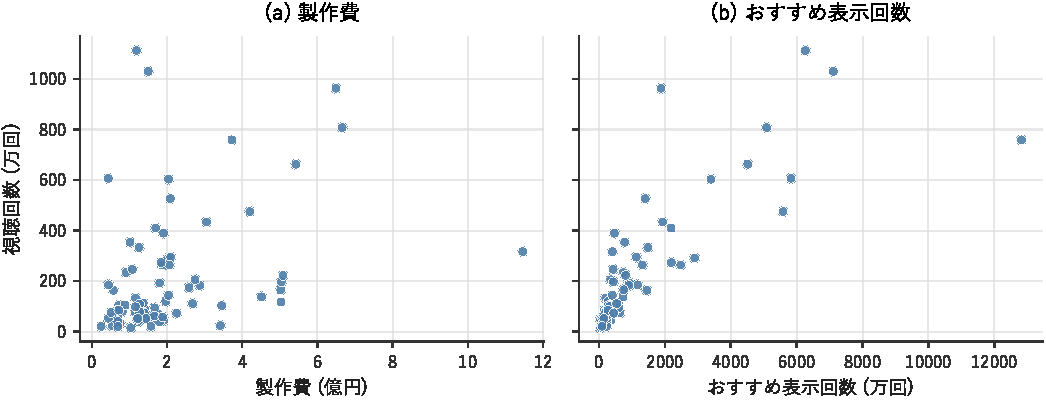
\includegraphics[width=\linewidth]{../figures/output/ch08_actual_scatter.pdf}
  \caption{80本の製作費／おすすめ表示回数と視聴回数の散布図. 1点が1作品を表す. 縦軸の尺度は共通だが, 横軸の単位と尺度は左右で異なる.}
  \label{fig:ch08-actual-scatter}
\end{figure}

では, 視聴回数とより強く連動しているのは, 製作費とおすすめ表示回数のどちらだろう.
2枚を並べて見比べても, どちらとも言えない.
横軸の単位も範囲も違う2枚の図では, 点の散らばり方をそのまま比べられないからだ.
おまけに, 散布図の印象は描き方ひとつで変わる.
同じデータでも, 縦軸を引き伸ばせば点の散らばりが縦に広がって関係が強そうに見えるし, 横軸を引き伸ばせば同じ理屈で弱そうに見える.
目で言えるのは, せいぜい「どちらも右上がり」までだ.

「一緒に動いている度合い」を, 目ではなく数で測れないだろうか.


\subsection{偏差の積から相関係数へ}

\subsubsection*{「一緒に動く」を偏差で捉える}

2つの変数$X$と$Y$が「一緒に動いている」とは, どういう状態のことだろうか.

もし$X$と$Y$が無関係なら, $X$が平均より大きい作品を選んでも, その作品の$Y$は大きいことも小さいこともあって, 規則性はない.
一方, $X$が平均より大きいときに$Y$も平均より大きい傾向があるなら, 二つは同じ方向に動いているといえる.
「一緒に動く」の中身は, 平均より上か下かという方向の一致らしい.

方向の一致なら, 第2章の偏差で捉えられそうだ.
ある値が平均より大きければ偏差は正, 小さければ負.
偏差の符号が, 平均より上か下かをそのまま表している.
そこで, $X$の偏差$(X - E[X])$と$Y$の偏差$(Y - E[Y])$を掛け合わせてみる.
両方が正なら, 積は正になる.
両方が負でも, 負$\times$負で積は正だ.
符号が食い違うときだけ, 積は負になる.
つまり偏差の積は, 一つのデータ点について「二つの変数が平均に対して同じ側にいるか, 逆の側にいるか」を符号で答える.

すべてのデータ点についてこの積を計算し, 平均をとってみる.
同じ側にいる点が多ければ平均は正に, 逆の側にいる点が多ければ負に傾く.
データ全体として同じ方向に動く傾向が強いのか, 逆方向の傾向が強いのかが, 1つの数値に集約される.

\subsubsection*{共分散の定義}

この考え方を式にしたものが\textbf{共分散}である.

\begin{defi}[]{共分散}{covariance}
2つの変数$X$, $Y$に対し, 共分散$\mathrm{cov}(X,Y)$を
\[
\mathrm{cov}(X,Y) = E[(X - E[X])(Y - E[Y])]
\]
と定義する.
\end{defi}

$(X - E[X])$は$X$の平均からのずれ, $(Y - E[Y])$は$Y$の平均からのずれで, その積の平均$E[\cdot]$をとっている.
第2章で学んだ分散の定義
\[
V(X) = E[(X - E[X])^2]
\]
と並べてみると, 分散は同じ変数の偏差どうしを掛けて平均したもの, 共分散は異なる変数の偏差どうしを掛けて平均したものだ.
分散の考え方を2変数に広げた量といえる.

共分散が正なら, $X$が大きいときに$Y$も大きい傾向がある.
負なら, $X$が大きいときに$Y$は小さい傾向がある.
0に近ければ, 同じ側と逆の側が打ち消し合っていて, どちらの傾向も強くない.

\subsubsection*{共分散の値は単位しだいで変わる}

符号が方向を表すなら, 値の大きさは連動の強さを表していそうだ.
確かめるために, 同じデータの単位だけを変えて, 共分散を計算し直してみる.
製作費を円で測るか, 万円で測るか.
円から万円への換算は1万で割るだけだが, 製作費の偏差も1万分の1になるから, 偏差の積も, その平均である共分散も1万分の1になる.
測っている作品は同じ, 視聴回数もそのままなのに, 製作費の単位を変えただけで, 共分散の値は1万分の1に変わってしまう.

値そのものがこれだけ動くと, 大きさの比較には使えない.
「製作費と視聴回数の共分散は1200, おすすめ表示回数と視聴回数の共分散は85」と並べられても, 製作費のほうが強く連動しているとは言えない.
1200と85の違いは, 連動の強さの違いではなく, 単位の違いを反映しているだけかもしれないからだ.

単位の影響を消して, 連動の強さだけを取り出したい.

\subsubsection*{ピアソンの相関係数}

第2章で学んだ標準偏差は, データが平均のまわりにどれくらい散らばるかを, データと同じ単位で表す量だった.
共分散を, $X$の標準偏差$\sigma_X$と$Y$の標準偏差$\sigma_Y$で割ってみる.
製作費を円から万円に変えると共分散は1万分の1になるが, 製作費の標準偏差も1万分の1になる.
分子と分母が同じだけ縮むので, 割った結果は変わらない.
単位の影響が, ここで消える.

こうして得られる量が\textbf{ピアソンの相関係数}$\rho$だ.

\begin{defi}[]{ピアソンの相関係数}{pearson-correlation}
2つの変数$X$, $Y$の標準偏差を$\sigma_X = \sqrt{V(X)}$, $\sigma_Y = \sqrt{V(Y)}$とする. ただし$\sigma_X > 0$かつ$\sigma_Y > 0$とする. ピアソンの相関係数$\rho_{XY}$を
\[
\rho_{XY} = \frac{\mathrm{cov}(X,Y)}{\sigma_X \, \sigma_Y}
\]
と定義する. $\rho_{XY}$は$-1$以上$1$以下の値をとる.
\end{defi}

分子は偏差の積の平均, 分母はそれぞれのばらつきの大きさの積だ.
単位の影響が分子と分母で打ち消し合うので, 製作費と視聴回数のペアでも, おすすめ表示回数と視聴回数のペアでも, 同じ尺度の上で値を読める.

別の見方もできる.
各変数をあらかじめ標準化して, 平均0, 標準偏差1に揃えてから共分散をとる, と考えてもよい.
標準化した変数を
\[
Z_X = \frac{X - E[X]}{\sigma_X}, \quad Z_Y = \frac{Y - E[Y]}{\sigma_Y}
\]
とすれば,
\[
\rho_{XY} = E[Z_X Z_Y]
\]
と書ける.
$Z_X$は「$X$が平均から標準偏差何個分離れているか」を表す, 単位のない量だ.
製作費が円でも万円でも, 標準偏差何個分かに直してしまえば同じ値になる.
相関係数は, 標準化した変数どうしの共分散だと言い直せる.

\subsubsection*{なぜ\texorpdfstring{$-1$}{-1}と\texorpdfstring{$1$}{1}の間に収まるのか}

定義には, $\rho_{XY}$が$-1$以上$1$以下の値をとると書いた.
積の平均なのだから, 平均から大きく離れた値どうしの積が重なれば, いくらでも大きくなりそうな気もする.
それでも$1$を超えられないのは, なぜだろうか.

手がかりは, $Z_X$と$Z_Y$の「食い違い」を測ってみることにある.
2つの量がどれだけ食い違っているかを見たいなら, 差を二乗して平均すればよい.
ずれを二乗して平均するという, 分散と同じ発想だ.
\[
E[(Z_X - Z_Y)^2] = E[Z_X^2] - 2E[Z_X Z_Y] + E[Z_Y^2]
\]
右辺は, $(a-b)^2 = a^2 - 2ab + b^2$という見慣れた展開の各項に, 期待値をとったものだ.
そして, 右辺の部品はすべて正体がわかっている.
$Z_X$は平均0だから, $E[Z_X^2]$は$Z_X$の分散そのものであり, 標準化で1に揃えてある.
$E[Z_Y^2]$も同じく1だ.
真ん中の$E[Z_X Z_Y]$は, さきほど見たとおり$\rho_{XY}$そのものだった.
代入すると,
\[
E[(Z_X - Z_Y)^2] = 1 - 2\rho_{XY} + 1 = 2(1 - \rho_{XY})
\]
となる.
左辺は二乗した量の平均だから, どんなデータでも0より小さくはならない.
すると右辺の$2(1 - \rho_{XY})$も0以上でなければならず, $\rho_{XY}$は1を超えられない.

では, ちょうど1になるのはどんなときか.
左辺が0になるとき, つまり$Z_X$と$Z_Y$の食い違いがまったくないときだ.
「相関係数が1」とは, 標準化した2つの変数が完全に重なっている状態のことだったのだ.

$-1$の側も同じ理屈で出る.
$Z_Y$の符号を反転した$-Z_Y$との食い違いを測れば, $E[(Z_X + Z_Y)^2] = 2(1 + \rho_{XY})$が0以上であることから, $\rho_{XY}$は$-1$を下回れない.
等号が成り立つのは$Z_X$と$-Z_Y$が完全に重なるとき, つまり2つの変数が完全に逆向きに連動しているときだ.
その間の値は, 完全な重なりと完全な逆向きのあいだの, 部分的な重なりの度合いを表している.

$-1$から$1$という範囲は, このように式から必然的に出てくる.
一方で, 標準偏差で割って尺度を揃えるという設計そのものは, 単位の違うペアどうしを比較したいという人間の都合で選ばれたものであって, 自然に決まる唯一の定義ではない.

\subsubsection*{\texorpdfstring{$\rho$}{ρ}の値と散布図の対応}

$\rho = 1$のとき, すべてのデータ点が完全に1本の右上がり直線の上に乗る.
$X$が増えれば$Y$も必ず増え, 例外は1点もない.
$\rho = -1$なら, 完全な右下がりの直線だ.

$|\rho|$が1から離れるにつれて, 点は直線から散らばり始める.
$\rho = 0.8$なら, 右上がりの傾向は明確だが, 直線からはみ出す点がちらほらある.
$\rho = 0.3$あたりになると, 右上がりの傾向はあるにはあるが, 散らばりが大きく, ぱっと見では判別しにくい.
$\rho = 0$では, 点の配置に方向性がなく, 雲のように広がる.
\cref{fig:ch08-correlation-examples}では, 軸の尺度を揃えてこの違いを並べた.

\begin{figure}[htbp]
  \centering
  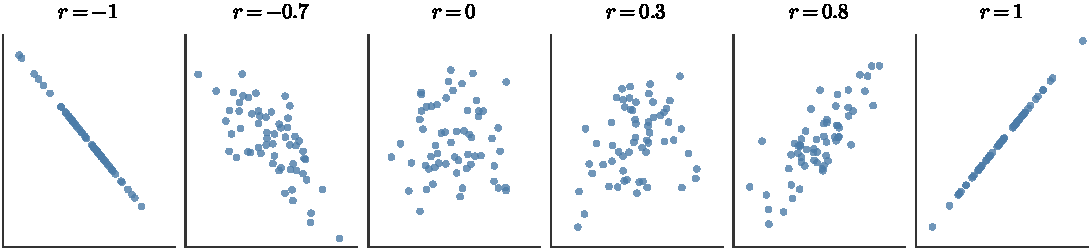
\includegraphics[width=\linewidth]{../figures/output/ch08_correlation_examples.pdf}
  \caption{相関係数 $r=-1,-0.7,0,0.3,0.8,1$ に対応する散布図. 各図は平均0, 標準偏差1に揃えた60点の合成データである.}
  \label{fig:ch08-correlation-examples}
\end{figure}

$|\rho|$が測っているのは, 点の並びが1本の直線にどれだけ近いか, である.

ただし, 直線への近さと直線の\textbf{傾き}は別の量だ.
ゆるやかな右上がりでも, 急な右上がりでも, 点が直線の上に乗っていれば$\rho = 1$になる.
相関係数が表すのは点がどれだけ直線に集まっているかであって, その直線がどれだけ急かではない.


\subsection{標本データからの計算手順}

ここまでの$\rho$は, 期待値$E[\cdot]$で書かれた母集団の性質だ.
実際に手元にあるのは, $n$個のデータの組$(x_1, y_1), (x_2, y_2), \ldots, (x_n, y_n)$である.
この標本から相関係数を計算する手順を追っていく.

なお, この計算には前提が2つある.
各データ点$(x_i, y_i)$が互いに独立に得られていることと, 調べたいのが2変数の直線的な関係であることだ.
前提から外れたデータで何が起きるかは, 本章の後半で確かめる.

\subsubsection*{手順}

計算は6つのステップで進む.
どのステップも, 前節の理論のどこかの部品に対応している.

\subsubsection*{ステップ1：平均を求める.}
\[
\bar{x} = \frac{1}{n} \sum_{i=1}^{n} x_i, \qquad \bar{y} = \frac{1}{n} \sum_{i=1}^{n} y_i
\]
これが「中心」の基準になる.

\subsubsection*{ステップ2：各データの偏差を求める.}
各$i$について$(x_i - \bar{x})$と$(y_i - \bar{y})$を計算する.
平均からどちらの方向にどれだけ離れているかが, ここで数値になる.

\subsubsection*{ステップ3：偏差の積を計算する.}
各$i$について$(x_i - \bar{x})(y_i - \bar{y})$を求める.
同方向のずれなら正, 逆方向なら負だ.
共分散の「中身」にあたる部分である.

\subsubsection*{ステップ4：偏差の積を合計し, 標本共分散を求める.}
\[
u_{xy} = \frac{1}{n-1} \sum_{i=1}^{n} (x_i - \bar{x})(y_i - \bar{y})
\]
分母は$n$ではなく$n-1$になっている.
第2章の脚注で触れた不偏分散と同じ理由で, 標本から母集団の共分散を偏りなく推定するために$n-1$で割る.

\subsubsection*{ステップ5：各変数の標本標準偏差を求める.}
\[
u_x = \sqrt{\frac{1}{n-1} \sum_{i=1}^{n} (x_i - \bar{x})^2}, \qquad u_y = \sqrt{\frac{1}{n-1} \sum_{i=1}^{n} (y_i - \bar{y})^2}
\]

\subsubsection*{ステップ6：標本相関係数を計算する.}
\[
r = \frac{u_{xy}}{u_x \, u_y}
\]
母集団の$\rho$に対応する標本からの推定値として, $r$を用いる.
分子と分母には同じ $n-1$ が含まれ, 比を取ると約分される.
したがって, $n-1$ で割る定義に揃えても相関係数の値は変わらない.

計算表を作って手で追うと, 偏差の符号がそのまま積の符号に現れる.
あわせて, 平均から大きく離れたデータの組は積の絶対値が大きく, 合計を強く引っ張る.
この性質は, 本章の後半でもう一度出てくる.

手順が揃ったところで, 実際のデータに当てはめる.


\subsection{三つの相関を比べる}

冒頭の問いに戻る.
視聴回数とより強く連動しているのは, 製作費とおすすめ表示回数のどちらか.
配信サービスの邦画作品の標本で, 実際に計算してみる.
3つの結果を先に\cref{fig:ch08-actual-correlations}へ並べる.

\begin{figure}[htbp]
  \centering
  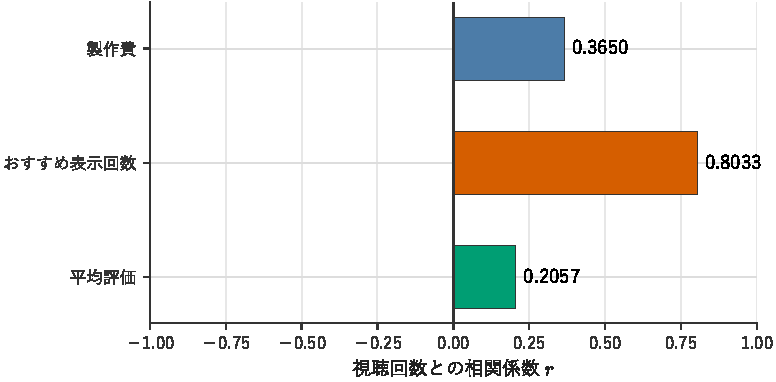
\includegraphics[width=0.8\linewidth]{../figures/output/ch08_actual_correlations.pdf}
  \caption{80本の実データから計算した, 視聴回数とのピアソンの標本相関係数. 3変数は単位が異なるが, 相関係数なら同じ尺度で比較できる.}
  \label{fig:ch08-actual-correlations}
\end{figure}

製作費と視聴回数の相関係数は, 前節の手順で計算すると $r = 0.3650$ となる.
弱から中程度の正の相関である.
散布図で見えていた右上がりの印象に, 数字がついた.
製作費の大きい作品ほど視聴回数も多い傾向はあるが, 点が1本の直線に沿って並ぶほどの強さではない.

同じ手順で, おすすめ表示回数と視聴回数の相関係数を計算すると, $r = 0.8033$ となる.
こちらは強い正の相関である.
冒頭では答えられなかった比較が, ここでは言い切れる.
単位も範囲もまるで違う2つのペアが, 同じ$-1$から$1$の物差しに乗っているからだ.
視聴回数との連動は, 製作費よりおすすめ表示回数のほうがはっきり強い.

もう一つ, 平均評価（5段階評価の平均値）と視聴回数の相関も計算してみると, $r = 0.2057$ で, こちらは弱い.
評価の高い作品ほど多く見られている, という素朴な期待は, 部分的にしか当たっていない.

3つの相関を並べると, 同じ「視聴回数との関係」でも, 相手の変数によって強さがかなり違う.
視聴回数は, 作品の中身や評判だけでなく, 配信側がどれだけ表示するかという配置に強く結びついているらしい.


\subsection{強い相関は因果を意味しない}

おすすめ表示回数と視聴回数の強い相関を見ると, おすすめ表示を増やせば視聴回数が伸びる, と読みたくなる.
だが, 相関係数が示しているのは, 二つの変数が連動しているという事実までだ.
連動していることと, 一方が他方の原因であることは, 別の話である.

有名な例がある.
夏になると, アイスクリームの売上が増える. 同じ時期に, 水難事故の件数も増える.
月ごとに集計すれば, アイスの売上と水難事故の件数には強い正の相関が出るはずだ.
だからといって, アイスを食べると溺れやすくなるわけではない.
両方を同時に動かしているのは\textbf{気温}という第三の変数だ.
気温が上がればアイスは売れるし, 海やプールに行く人が増えて事故も増える.

このように, 背後の共通の原因が二つの変数を同時に動かしているために生まれる相関を\textbf{擬似相関}と呼ぶ.
共通の原因にあたる変数は\textbf{交絡因子}という.
アイスと水難事故なら誰も因果を疑わないが, もっともらしい組み合わせで同じ構造が現れると, 気づくのは難しい.

おすすめ表示回数と視聴回数の場合は, 擬似相関とはまた別の難しさもある.
「おすすめに表示されたから視聴された」のか, 「よく視聴された作品が, 人気があると判断されてさらに表示された」のか.
どちらの向きでも, 観測される相関は同じ正の値になる.
相関係数は連動の強さを測るだけで, どちらが先でどちらが後か, という向きの情報を含んでいない.

相関からわかるのは, 「関係がありそうだ」という手がかりまでだ.
因果を主張するには, 第三の変数の影響を断つ設計（たとえば実験や条件の統制）や, 時間の前後関係の確認が別に必要になる.
この点は第10章で改めて扱う.


\subsection{相関係数だけではわからないこと}

相関係数は, 二つの変数の散らばり方を1つの数値に要約している.
第2章で見たとおり, 要約すれば落ちる情報がある.
そして, 落ちた情報が結論を左右することもある.

\subsubsection*{\texorpdfstring{$\rho = 0$}{ρ = 0}でも関係がないとは限らない}

$Y = X^2$という関係を考えてみる.
$X$が$-3$から$3$まで対称に散らばっているとすると, $X$が負のときも正のときも, 絶対値が大きければ$Y$は大きい.
散布図を描けば, きれいなU字型が現れる.
$X$を決めれば$Y$が決まるのだから, 関係としてはこの上なく強い.
ところが, 相関係数を計算すると, ほぼ0になる.
$X$が負の側では偏差の積が負に, 正の側では正になり, 対称に散らばっているせいで打ち消し合うからだ.

前に見たとおり, 相関係数が測っているのは, 点の並びが直線にどれだけ近いかだった.
U字のような曲がった関係は, どれだけ強くても$\rho$の値には現れない.
$\rho$が0に近いことから言えるのは「直線的な関係が見当たらない」までで, 「関係がない」ではない.

\subsubsection*{たった1点で値が変わる}

次の10個のデータ点で相関係数を計算すると, $r \approx 0.05$になる.
\[
(1,6),\; (2,1),\; (3,7),\; (4,5),\; (5,8),\; (6,3),\; (7,10),\; (8,9),\; (9,2),\; (10,4)
\]
\cref{fig:ch08-outlier}の左側を見ても, 点はほぼランダムに散らばっていて, 直線的な関係は見当たらない.

ここに, 他の点からかけ離れた$(22, 22)$という1点を追加して, 11個で計算し直すと, $r \approx 0.76$になる.
ほぼ無相関だった10点が, 1点増えただけで, かなり強い正の相関に読める数値に変わった.

\begin{figure}[htbp]
  \centering
  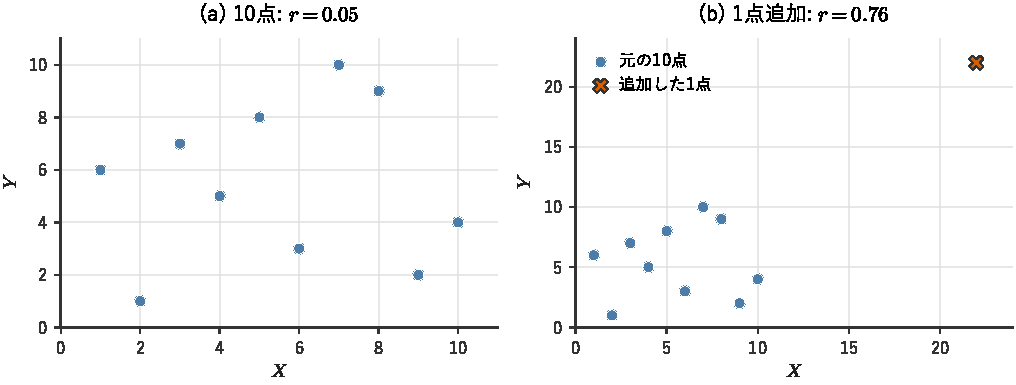
\includegraphics[width=0.9\linewidth]{../figures/output/ch08_outlier.pdf}
  \caption{外れ値を加える前後の散布図. 左は10点で $r=0.05$. 右は同じ10点に $(22,22)$ を加えた11点で $r=0.76$. 元の10点を読み取れるよう, 左右で軸の範囲を変えている.}
  \label{fig:ch08-outlier}
\end{figure}

原因は, 計算手順の節で見た偏差の積の性質にある.
$(22, 22)$はどちらの変数でも平均から大きく離れているから, この1点の偏差の積が, 他の10点の積の合計よりはるかに大きい.
$r \approx 0.76$という値は, 事実上この1点が決めている.

数値だけを見ていたら, そのことには気づけない.
散布図には, 10点の無秩序な散らばりと, ぽつんと離れた1点が, そのまま見えている.

\subsubsection*{部分と全体で向きが逆になる}

ある大学の2つの学部で, 勉強時間と試験の成績の関係を調べたとする.
学部Aの学生30人で計算すると$r = 0.7$, 学部Bの学生30人でも$r = 0.6$.
どちらの学部でも, 勉強時間が長い学生ほど成績がよい.
ところが, 2学部の60人をまとめて計算し直すと, $r \approx -0.3$という負の値になることがある.

\begin{figure}[htbp]
  \centering
  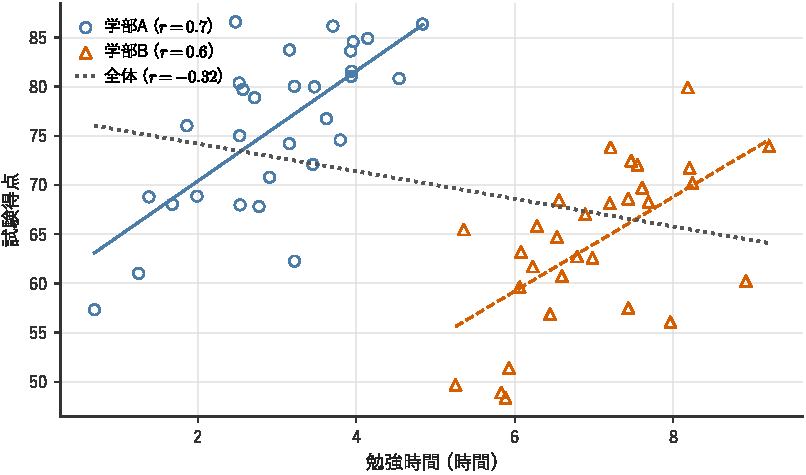
\includegraphics[width=0.8\linewidth]{../figures/output/ch08_simpson.pdf}
  \caption{シンプソンのパラドックスを示す合成データ. 学部Aと学部Bは各30人で, 群内の相関はそれぞれ $r=0.700$, $r=0.600$. 2群をまとめると $r=-0.316$ になる. 点の形と線種でも群と回帰直線を区別した.}
  \label{fig:ch08-simpson}
\end{figure}

原因は, 2つの群の平均の位置にある.
学部Aが平均的に勉強時間が短く成績の高い集団で, 学部Bが平均的に勉強時間が長く成績の低い集団だったとする.
60人まとめて計算すると, 偏差の基準になる平均は2つの群の中間に来る.
すると学部Aの学生の多くは「勉強時間が平均より短く, 成績は平均より高い」側に, 学部Bの学生の多くはその逆側に入り, 偏差の積は負に傾く.
各学部の中の右上がりの傾向より, 群と群の位置関係のほうが強く効いてしまうのだ.

この現象は\textbf{シンプソンのパラドックス}と呼ばれる.
集計の仕方しだいで, 相関の向きまで変わりうるという例である.
そしてここでも, \cref{fig:ch08-simpson}を見れば, 右上がりの2つのかたまりが離れた場所に並んでいる様子がそのまま見えている.

\vspace{1em}

U字も, 離れた1点も, 2つのかたまりも, 相関係数の数値だけでは見分けがつかない.
散布図には, どれもそのまま見えている.
散布図だけでは連動の強さを比べられなかったように, 相関係数だけでは散らばりの姿がわからない.
散布図で姿を確かめ, 相関係数で強さを測る. どちらか一方では足りない.

\begin{mybox}{カール・ピアソンと相関係数の歴史}
相関係数を体系的に定式化したのは, イギリスの統計学者カール・ピアソン（1857--1936）である.\footnotemark
ピアソンは, フランシス・ゴルトンが親子の身長データから見出した「回帰」の考え方を数学的に整備し, 相関係数の計算法を確立した.

しかし, ピアソンは優生学の熱心な推進者でもあった.
彼が相関係数を発展させた動機の一つは, 遺伝的特徴の親子間の「関係の強さ」を測ることにあり, その成果は優生政策の正当化にも使われた.
相関係数という数式そのものは中立でも, どんな問いに対して, どんな意図で使うかによって, 結果の意味はまったく変わる.

統計の手法を学ぶときは, 「それで何ができるか」だけでなく, 「それがどう使われてきたか」にも目を向ける価値がある.
\end{mybox}
\footnotetext{%
相関係数の定式化は Pearson, K. (1896). Mathematical Contributions to the Theory of Evolution. III. Regression, Heredity, and Panmixia. \textit{Philosophical Transactions of the Royal Society of London. Series A}, 187, 253--318.}


\subsection{測れたものと, まだ測れていないもの}

本章では, 二つの量が一緒に動く度合いを, 偏差の積から組み立てた.
偏差の積の平均が共分散になり, それぞれの標準偏差で割ると, 単位によらない$-1$から$1$の尺度になる.
単位の違う3つの変数について視聴回数との相関を並べ, おすすめ表示回数がいちばん強く, 製作費は弱いながらも正, 平均評価はさらに弱い, という順序まで確かめられた.

ここで言えたのは, 連動の向きと強さまでだ.
おすすめ表示が視聴回数を押し上げているのか, 視聴された作品がさらに表示されやすくなるのか, その向きは相関係数からは決められなかった.
そして, 製作費と視聴回数に弱い正の相関があるとわかっても, 製作費を増やしたら視聴回数がどれだけ変わるのか, という量については, まだ何も言えていない.
